\section{Implementation} Second step of adopting the automation practices is setting up the processes using chosen tools. The implementation goal is to pro


\subsection{Containerization}  I have adopted the containerization using Docker for a use in CI/CD pipeline. The Dockerfile simply contains the instruction for building a Docker images. It composed of specific commands which tell how to build the image. A Docker image is a read-only file containing a set of instructions. When these instructions are executed, a Docker container is created. 
%https://www.simplilearn.com/tutorials/docker-tutorial/what-is-dockerfile


\begin{lstlisting}[language=Octave, caption=Dockerfile]
FROM node:latest as build
WORKDIR /app
COPY package*.json ./
RUN yarn
COPY ./ .
RUN yarn run build

FROM nginx
RUN mkdir /app
COPY --from=build /app/dist /app
COPY nginx.conf /etc/nginx/nginx.conf
\end{lstlisting}

\noindent Dockefile showed on listing 5.1 contains installing dependencies on the fifth row and application bundling on the six's row using Yarn and also adding Nginx configuration from the \texttt{nginx.conf} file on the last row, which defines parameters like hostname, listen port and others.



\subsection{CI/CD pipeline configuration} CI/CD pipeline is a set of steps that are executed when the pipeline was triggered.\\
Listing 5.2 shows all the stages of the CI/CD pipeline. First two stages where configured by Ing. Oldřich Malec with the first setup of the frontend projects. Download stage installs all the dependencies required for the application run. Codestyle stage provides linting of the source code. Other three stages I have implemented in this thesis.
\begin{lstlisting}[language=Octave, caption=Gitlab CI/CD stages]
stages:
  - download
  - codestyle
  - test
  - build
  - deploy
\end{lstlisting}

\noindent GitLab provides the visualization of the pipeline steps and allows to execute any steps manually as well as monitor the log of any job from the pipeline. Figure 5.1 shows how the passed pipeline looks in the BI-DBS portal frontend.

\begin{figure}[ht]
\centering
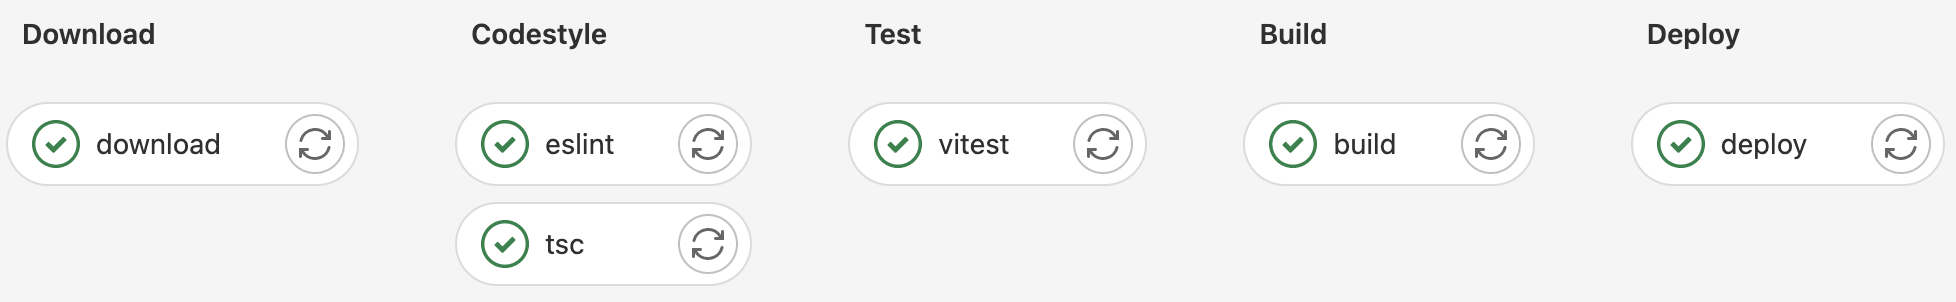
\includegraphics[scale=0.377]{../png/pipeline.png}
\caption{CI/CD pipeline in GitLab}
\end{figure}

\noindent The pipeline stages are executed from left to right and if any of the stages fails all the other ones will be skipped. It helps to avoid pointless running of jobs, because the stages are put in the way that they depend on the result of the previous ones. 




\subsubsection{Test} Test stages contains one job which I have named vitest, because it executes unit tests implemented using Vitest framework which will be introduced in the six's chapter. For running the tests I have used Yarn, which provides the tests execution by running just one command which is added to script section on the line fifteen of the listing 5.3. 
\begin{lstlisting}[language=Octave, caption=Test stage in the CI/CD pipeline]
.image_template: &image
  image: $CI_REGISTRY/ict/images/alpine/ci:3.16
  before_script:
    - apk add -U nodejs yarn

.cache_pull_template: &cache
  key: $CI_COMMIT_REF_SLUG
  paths:
    - node_modules/
    
vitest:
  <<: *image
  stage: test
  script:
    - yarn run test
  cache:
    <<: *cache

\end{lstlisting}

\noindent For the tests execution setup in the pipeline I have used image and cache pull templates, which were already prepared and used for the download and codestyle stages.




\subsubsection{Build} Build stage is focused on building an image and adding it to the GitLab container registry of the project. I have used the faculties image containing buildah and buildah itself for the script which is shown in listing 5.4. Command from the row number seven will create the image and the next command from the row number eight will upload it to GitLab registry.\\

\begin{lstlisting}[language=Octave, caption=Build stage in the CI/CD pipeline]
build:
  image: $CI_REGISTRY/ict/images/buildah:v1
  stage: build
  variables:
    IMAGE_TAG: $CI_REGISTRY_IMAGE:$CI_COMMIT_REF_NAME
  script:
    - buildah build --squash --tag $IMAGE_TAG -f Dockerfile
    - buildah push $IMAGE_TAG
  only:
    - devtest
\end{lstlisting}

\noindent The last two rows of the listing define the only branch for which this job will be executed. The BI-DBS frontend does not have a production version yet. Therefore I have decided to create the environment for deploying the application for testing during the development process. For that reason I have created a branch named devtest, any changes pushed to which will be automatically built and deployed.


\subsubsection{Deploy} When it comes to deploy stage, it means that the application when though all the previous pipeline stages and application is ready to be deployed. The deployment process of the CI/CD pipeline is composed of execution of deployment script from the server. For the connetion to the server GitLab uses CI/CD variable which allow securely storing sensetive data, which need to be used in the pipeline like for example deployment user showed on line number six of listing 5.5.


\begin{lstlisting}[language=Octave, caption=Deploy stage in the CI/CD pipeline]
deploy:
  stage: deploy
  dependencies:
    - build
  script:
    - ssh -A "${DEPLOYER_IP_ADDRESS}" -l ${DEPLOYER_USER} 'bash deploy-dbs-frontend.sh'
  only:
    - devtest
\end{lstlisting}


\noindent Deployment script contains few steps such as pulling Docker image from the GitLab created in the build stage, then creating and running a container and logging the container running. The configuration of this process is securely stored on the server.